\documentclass[11pt,a4paper]{article}
\usepackage{geometry}
\geometry{a4paper, margin=1in}
\usepackage{amsmath} % for math formulas
\usepackage{booktabs} % for better tables

\usepackage{graphicx}
\usepackage{hyperref}

\title{AIML231 Assignment 3 Report}
\author{Shemaiah Rangitaawa | \texttt{300601546}}
\date{May 2024}

\begin{document}

\maketitle
\begin{abstract}
    This report analyzes the application of machine learning techniques across three domains: linear regression, clustering, and neural
    networks. It assesses vehicle fuel efficiency using linear regression on the Auto MPG dataset, compares K-means and hierarchical clustering
    on a synthetic dataset, and explores neural network capabilities with the famous Handwritten Digits dataset.
\end{abstract}

\section{Linear Regression}
\subsection{Exploratory Data Analysis (EDA)}

\begin{figure}[ht]
    \centering
    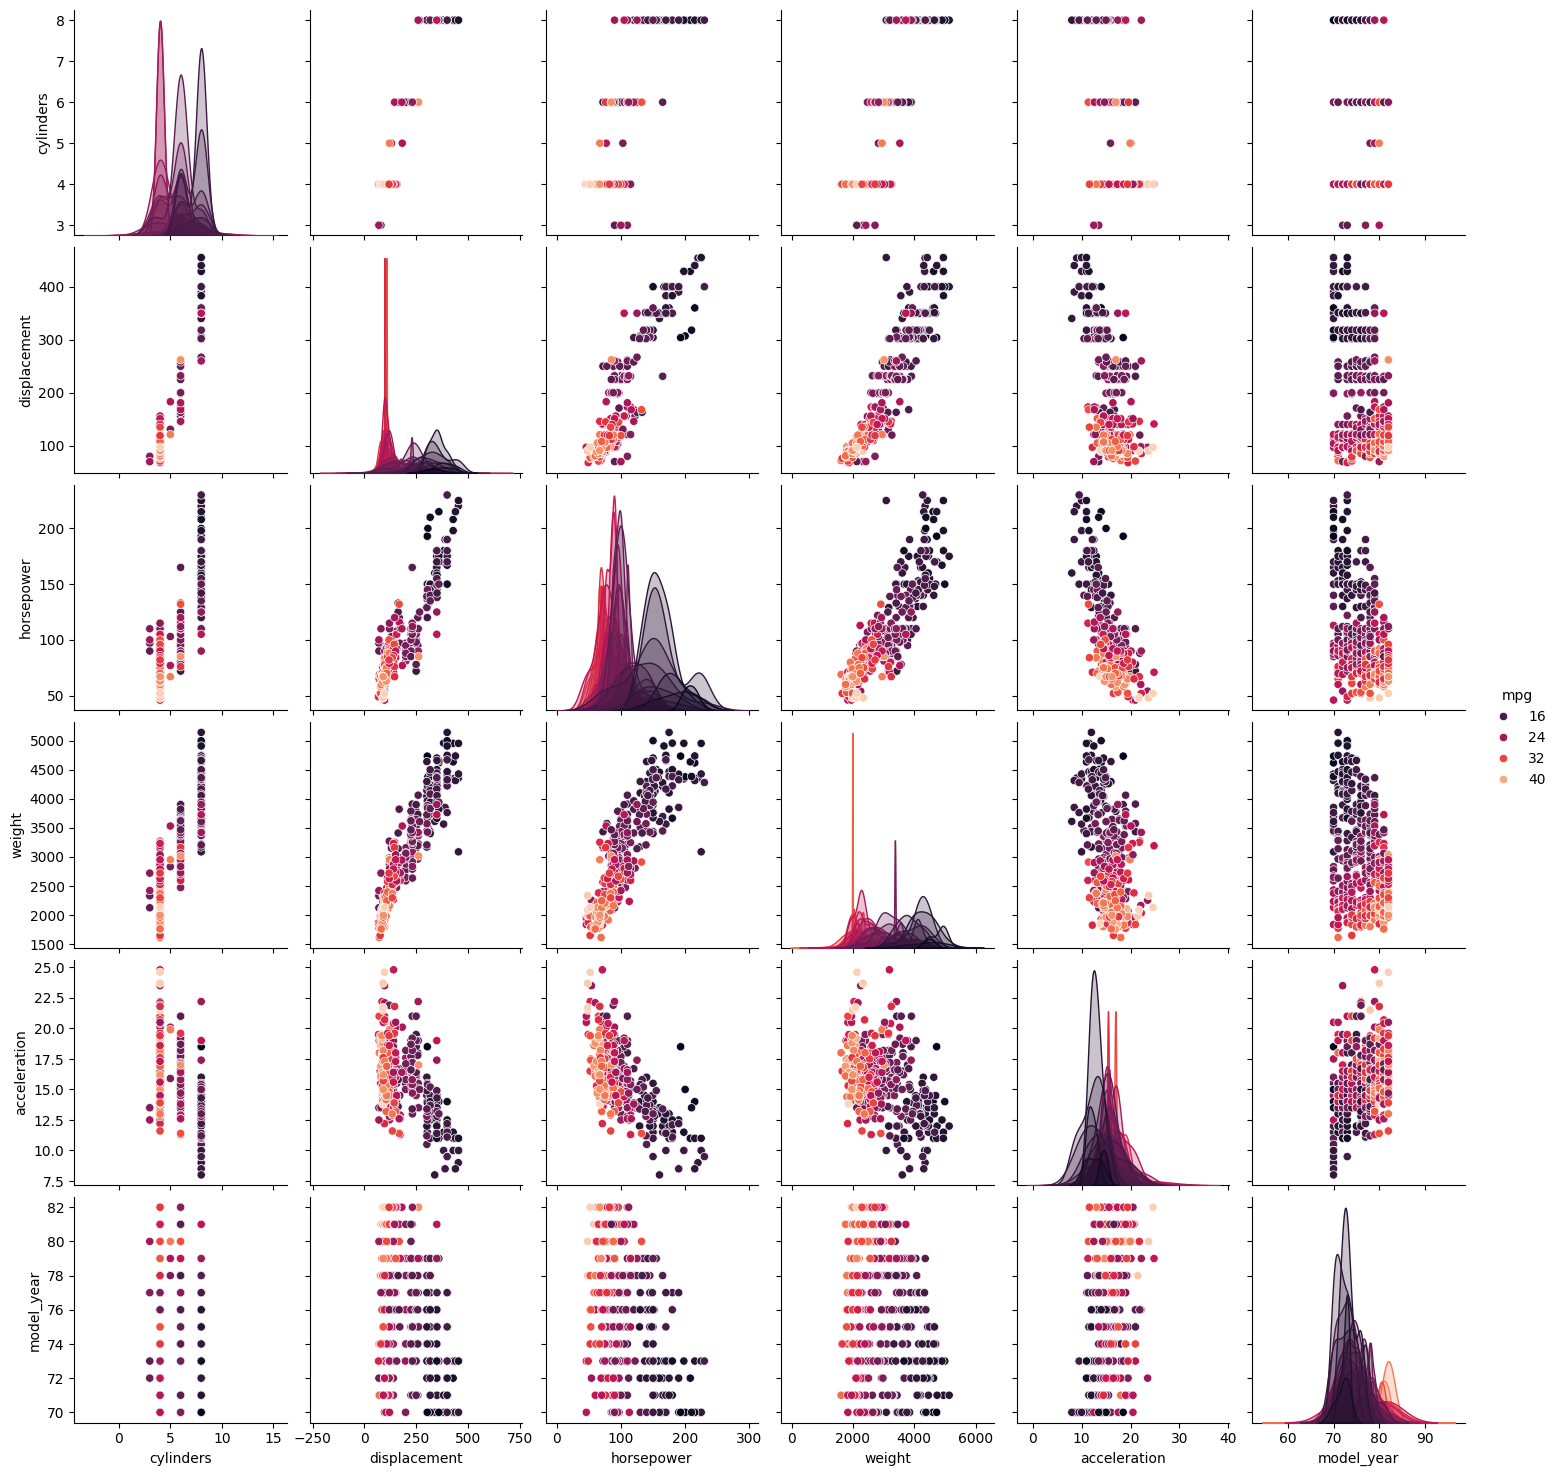
\includegraphics[width=0.75\textwidth]{images/pairplot.png}
    \caption{Pair plot of MPG against various vehicle attributes}
    \label{fig:mpgpairplot}
\end{figure}

The Auto MPG dataset contains 398 instances and 8 features, with 2 categorical and 6 numerical attributes.
The pair plot in Figure \ref{fig:mpgpairplot} illustrates the relationship between MPG and other vehicle characteristics,
highlighting potential correlations and patterns. Notable observations include:

\begin{itemize}
    \item \textbf{Vehicle Weight and MPG:} There is a clear negative correlation between MPG and vehicle weight. As weight increases, MPG decreases, suggesting that heavier cars tend to have lower fuel efficiency.
    \item \textbf{MPG and Displacement:} Similarly, there's a strong negative correlation between MPG and engine displacement. Larger engine sizes are associated with lower MPG.
    \item \textbf{MPG and Horsepower:} The scatter plot shows a negative correlation between MPG and horsepower. Vehicles with higher horsepower generally have lower MPG.
    \item \textbf{Model Year and MPG:} There is a trend indicating that newer models tend to have better MPG, showing an improvement in fuel efficiency over time.
\end{itemize}

\begin{figure}[ht]
    \centering
    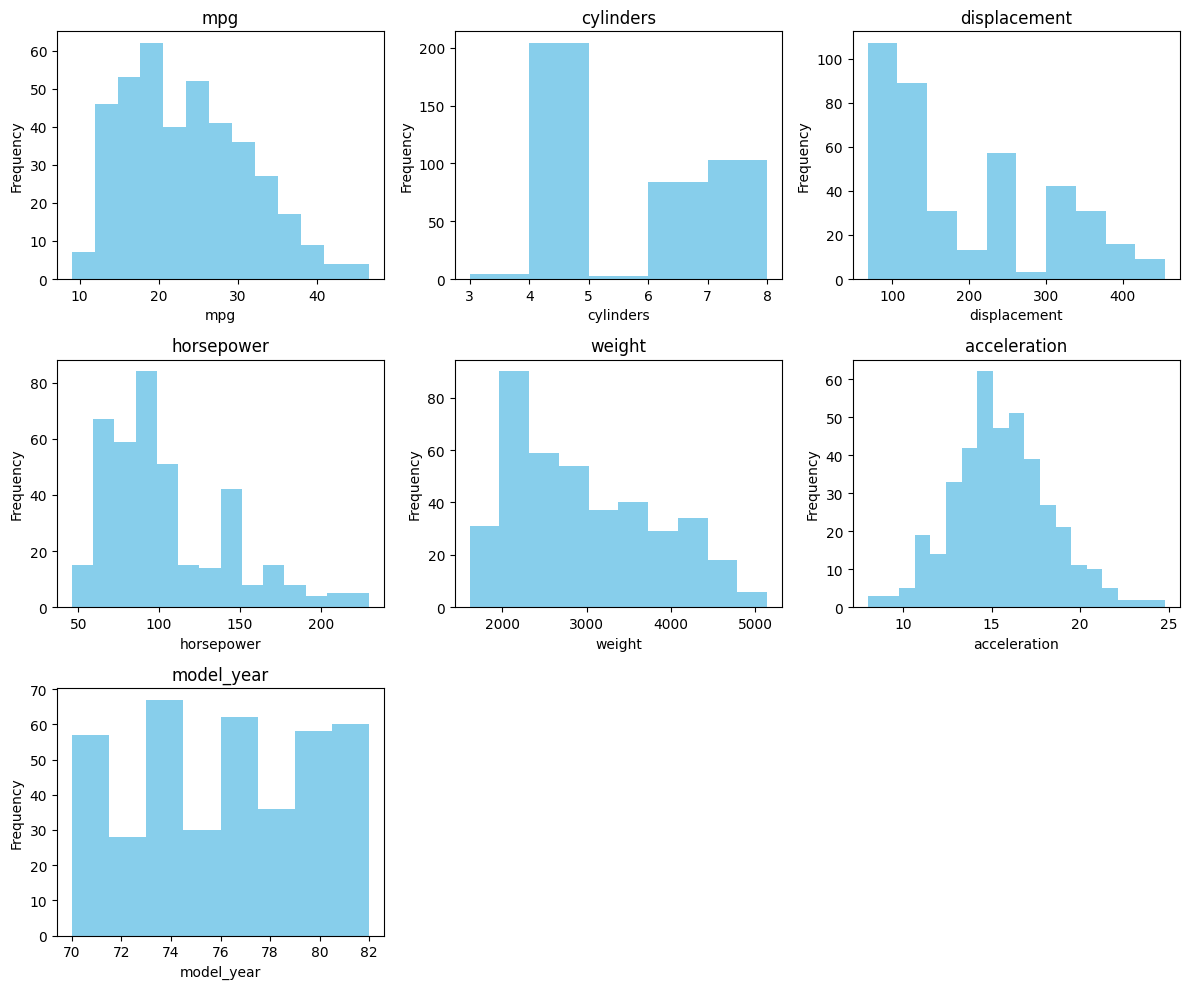
\includegraphics[width=0.75\textwidth]{images/hist.png}
    \caption{Pair plot of MPG against various vehicle attributes}
    \label{fig:mpghistogram}
\end{figure}

\noindent
Analyzing the histogram plots in Figure \ref{fig:mpghistogram} we see that MPG data is right-skewed, indicating many vehicles have high fuel efficiency,
likely newer or technologically advanced models. Predominantly, these vehicles feature 4-cylinder engines, which do tend to have lower displacement and horsepower, enhancing MPG.
This trend suggests a move towards engine designs optimized for fuel efficiency. A strong correlation exists between engine displacement,
horsepower, and the number of cylinders, crucial for modeling their impact on fuel efficiency.
\vspace*{11pt}

\noindent
Vehicle weight distribution is also right-skewed, with fewer heavy vehicles, reinforcing the negative relationship between weight and MPG.
Acceleration displays a normal distribution, suggesting it varies less between vehicles and is less influential on fuel efficiency
compared to engine size or weight.
\vspace*{11pt}

\noindent
Additionally, the increase in vehicle models from the early 1970s to the 1980s likely reflects advances in automotive technology
and shifts in market availability, reflecting improvements in fuel efficiency and emission standards important for charting
historical progress in vehicle technology.

\subsection{Preprocessing Methodology}
There is a total of four categorical variables in the dataset:
\begin{itemize}
    \item \textbf{Cylinders} (e.g., 4, 6, 8), indicating engine types.
    \item \textbf{Model Year}, representing different model groups each year.
    \item \textbf{Origin}, denoting the region or country of manufacture.
    \item \textbf{Model Name}, classifying car models.
\end{itemize}
\textbf{Encoding Methods:}
\begin{itemize}
    \item \textbf{Cylinders} are encoded using the Ordinal method to reflect the natural order (4 cylinders, 6 cylinders, etc.).
    \item \textbf{Model Year} and \textbf{Origin} are encoded using One-hot encoding. This approach converts each category into a unique feature,
          enabling the independent evaluation of each feature's impact.
    \item \textbf{Model Name}: Encoded using target encoding to manage high cardinality and \\ incorporate the relationship with the target variable (\texttt{MPG}) efficiently.
\end{itemize}
\textbf{Missing Values and Imputation Strategy:}\\
There are six missing entries in the \textit{Horsepower} column. To maintain data integrity and continuity for the analyses,
these values have been imputed using a mean imputation strategy. This approach involves replacing missing values with the
average \textit{Horsepower} across all available data points.

\vspace*{11pt}
\noindent \textbf{Justification:}\\
The decision to apply mean imputation is supported by several considerations:
\begin{itemize}
    \item \textbf{Preservation of Data Distribution:} Mean imputation helps maintain the original distribution of the data,
          such that the central tendency and variance remain consistent. This is important for any subsequent statistical analysis or
          modeling where the integrity of data distribution impacts the accuracy of results.
    \item \textbf{Simplicity and Efficiency:} This technique is straightforward and computationally \\ efficient, making it an
          attractive choice when quick and effective solutions are required. It does not require complex calculations or
          algorithms (unlike KNN imputation), enabling rapid preprocessing of data.
    \item \textbf{Suitability for Linear Models:} Linear models rely on the assumption of minimal bias in the input data.
          Mean imputation reduces the risk of bias that can be introduced by outliers or more intricate methods of handling missing data.
          By filling missing entries with the mean, we ensure that each feature's average value reflects the typical data point,
          therfore minimizing distortions in the model’s outcome.
\end{itemize}
\newpage
\subsection*{Linear Model Implementation}
The linear regression model was developed using the PyTorch library, leveraging its \texttt{nn.Module}.
Specifically, the implementation uses a subclass of \texttt{nn.Module} to integrate a single \texttt{nn.Linear} layer.
This layer is dynamically configured to manage its learnable parameters.
\subsection*{Training}
Training the model involved several key components:
\begin{itemize}
    \item \textbf{Loss Function:} The Mean Squared Error (MSE) loss function is utilized to highlight and correct larger prediction errors, enhancing the robustness of the regression model.
    \item \textbf{Optimizer:} Stochastic Gradient Descent (SGD) serves as the optimizer with a learning rate set at 0.01. This choice is dictated by SGD's proven effectiveness and simplicity in various machine learning applications.
    \item \textbf{Training Process:} The model undergoes a training regimen spanning 4000 epochs. Each epoch consists of:
          \begin{enumerate}
              \item A forward pass to compute predictions.
              \item Loss calculation to evaluate the error magnitude.
              \item A backward pass to adjust the model's parameters using the computed gradients.
          \end{enumerate}
\end{itemize}

\subsection{Model Coefficients}
A complete table of coefficients is available in the submission to the ECS page. Here are the coefficients for several key features:

\begin{table}[ht]
    \centering
    \begin{tabular}{lc}
        \toprule
        Feature                & Coefficient \\
        \midrule
        Cylinders              & -0.003312   \\
        Weight                 & 6.73896     \\
        Miles Per Gallon (MPG) & -0.001937   \\
        Horsepower             & -0.059632   \\
        Acceleration           & 0.104624    \\
        \bottomrule
    \end{tabular}
    \caption{Coefficients of key features}
    \label{tab:coefficients}
\end{table}
\noindent
Each coefficient indicates the feature's impact on the output, with negative values indicating a decrease and positive values an increase in output as the feature value rises.

\subsection{Performance Metrics}

The model's performance was quantified using the following metrics:

\begin{itemize}
    \item \textbf{Test Mean Squared Error (MSE)}: Achieved a value of around 0.75, indicating high predictive accuracy with minimal error between the predicted and actual values.
    \item \textbf{Test R-squared (R²)}: The value was around 0.98, meaning 98\% of the variance in the dependent variable is explained by the independent variables, showcasing an excellent fit of the model to the data.
\end{itemize}
\noindent
The metrics validate the strong predictive performance of the model, as evidenced by the low MSE and high R² values.

\section {Clustering}
\subsection*{Dataset Generation}
As per the assignment brief, the dataset used for clustering was generated synthetically using the \texttt{make\_blobs} function from \texttt{sklearn.datasets} module.
Specifically:
\begin{table}[ht]
    \centering
    \begin{tabular}{lc}
        \hline
        \textbf{Parameter}              & \textbf{Value} \\
        \hline
        Number of samples               & 300            \\
        Number of centers (clusters)    & 3              \\
        Number of features per sample   & 4              \\
        Random seed for reproducibility & 231            \\
        \hline
    \end{tabular}
    \caption{Parameters used in the generation of the synthetic dataset}
    \label{tab:dataset_params}
\end{table}

\subsection{Comparison of Linkage Methods in Hierarchical Clustering}

\begin{figure}[ht]
    \centering
    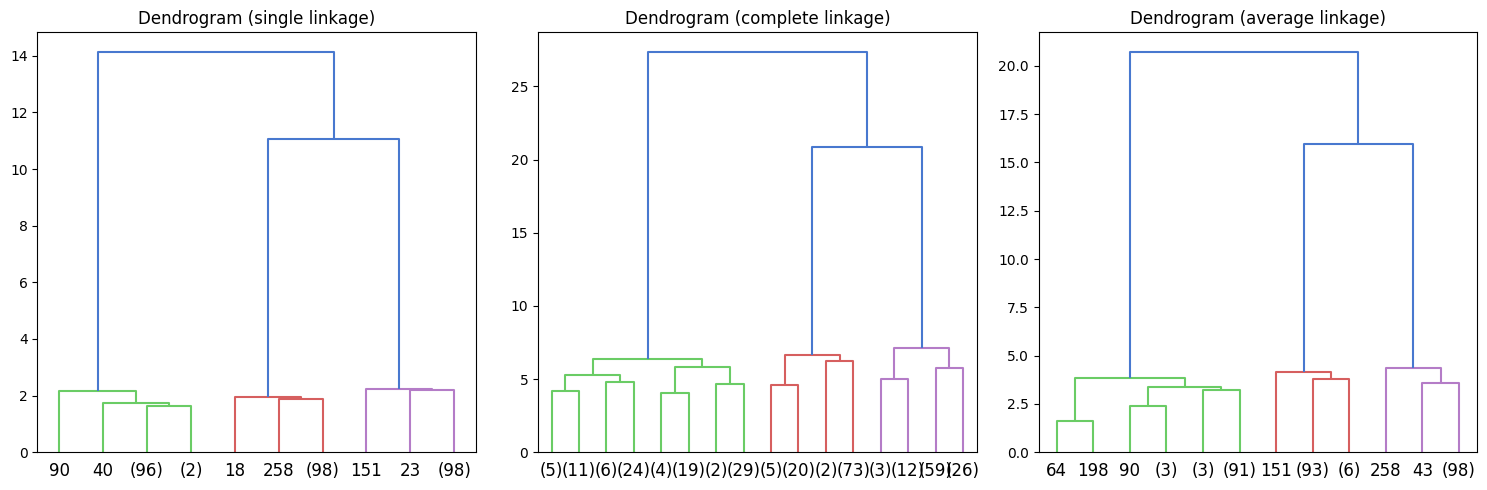
\includegraphics[width=1\textwidth]{images/dendrogram.png}
    \caption{Dendrogram illustrating hierarchical clustering using different linkage methods}
    \label{fig:dendrogram}
\end{figure}

\noindent The Python library \texttt{matplotlib} and \texttt{scipy} were used to generate and visualize dendrograms for each linkage method.

\subsection*{Single Linkage}
Single linkage shows significant chaining, with elongated clusters that incorporate several
other clusters at a high linkage distance, indicative of a less homogeneous cluster formation.

\subsection*{Complete Linkage}
Complete linkage creates more balanced and compact clusters, with a uniform size across
clusters. This method is less influenced by outliers, leading to tighter and more homogeneous groups.

\subsection*{Average Linkage}
Average linkage produces a balance between the extremes of single and complete linkage,
leading to clusters that are compact but flexible, accommodating for variation within the data points.

\subsection{Comparison of Hierarchical and K-means Clustering}

\subsection*{Hierarchical Clustering}
Hierarchical clustering works well in handling complex cluster structures, accommodating a variety of data distributions without needing predefined cluster numbers.
This enhances interpretability through dendrogram analysis. However, the method's computational intensity grows with data size, and it can be sensitive
to noise and outliers, particularly in methods like single linkage, which could degrade cluster quality.

\subsection*{K-means Clustering}
K-means clustering is efficient and effective for large datasets, quickly converging to cluster centroids.
It uses silhouette scores for evaluating cluster quality, producing the optimal cluster count and assessing
separation and cohesion. However, it requires predefined cluster numbers and is vulnerable to local minima,
which could lead to suboptimal clustering if initial centroids are poorly chosen.

\section{Neural Networks}
\subsection*{Network Architecture | Design of the \texttt{MLPNN} Class}

In designing the \texttt{MLPNN} class, I tried to create a versatile and scalable multi-layer perceptron suitable for many machine learning tasks.
The class allows for dynamic configuration of the network’s architecture through a layer parameter, where each element specifies the
number of neurons in a hidden layer.

The architecture uses \texttt{nn.ModuleList} for managing an arbitrary number of hidden layers,
enhancing the model's flexibility. An important design decision was to exclude an activation function from the output layer,
optimizing the network for classification tasks by outputting logits for use with cross-entropy loss.
This ensures the outputs are suitable for probability calculations.

\subsection{Training Output}
The training process involved 15 epochs, with a learning rate of \texttt{0.001} and a batch size of \texttt{64}.
\begin{verbatim}
                    Epoch 1: Loss = 2.102, Accuracy = 53%
                    Epoch 2: Loss = 1.586, Accuracy = 84%
                    Epoch 3: Loss = 1.022, Accuracy = 90%
                    Epoch 4: Loss = 0.649, Accuracy = 91%
                    Epoch 5: Loss = 0.454, Accuracy = 93%
                    Epoch 6: Loss = 0.353, Accuracy = 94%
                    Epoch 7: Loss = 0.288, Accuracy = 95%
                    Epoch 8: Loss = 0.244, Accuracy = 95%
                    Epoch 9: Loss = 0.212, Accuracy = 96%
                    Epoch 10: Loss = 0.188, Accuracy = 96%
                    Epoch 11: Loss = 0.170, Accuracy = 97%
                    Epoch 12: Loss = 0.158, Accuracy = 97%
                    Epoch 13: Loss = 0.142, Accuracy = 98%
                    Epoch 14: Loss = 0.132, Accuracy = 97%
                    Epoch 15: Loss = 0.122, Accuracy = 98%
\end{verbatim}
\newpage
\subsection{Test Output}
The model was evaluated on the test set, yielding an accuracy of \texttt{95.83} percent.
\begin{figure}[ht]
    \centering
    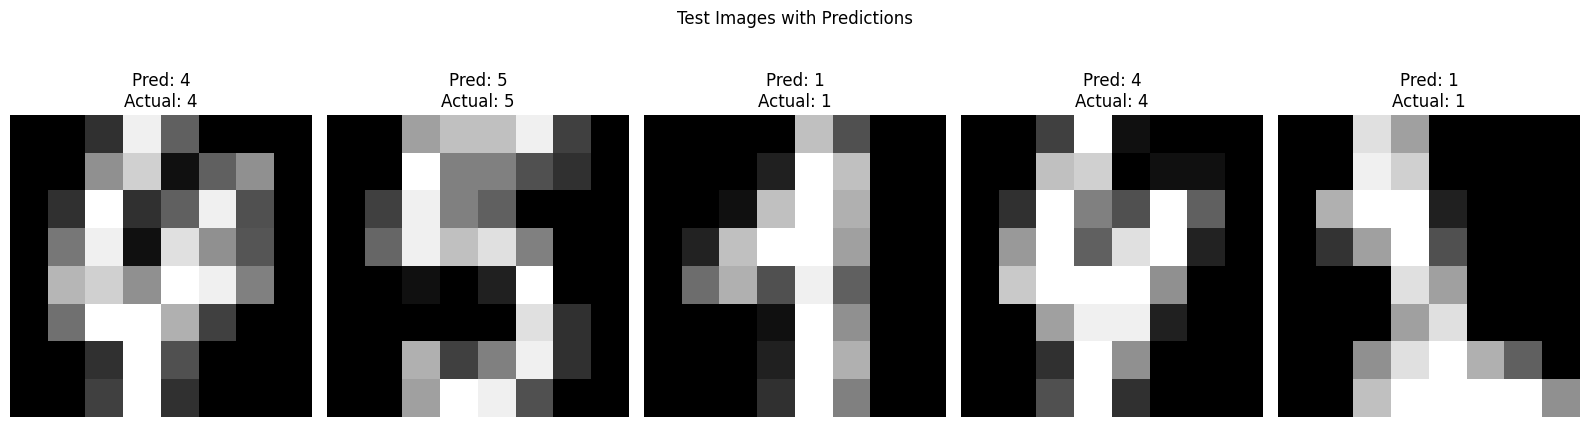
\includegraphics[width=1\textwidth]{images/test_images.png}
    \caption{Images with predicted and actual labels}
    \label{fig:test_images}
\end{figure}

\subsection{Comparison of the Effects of Different Activation Functions}
\begin{figure}[ht]
    \centering
    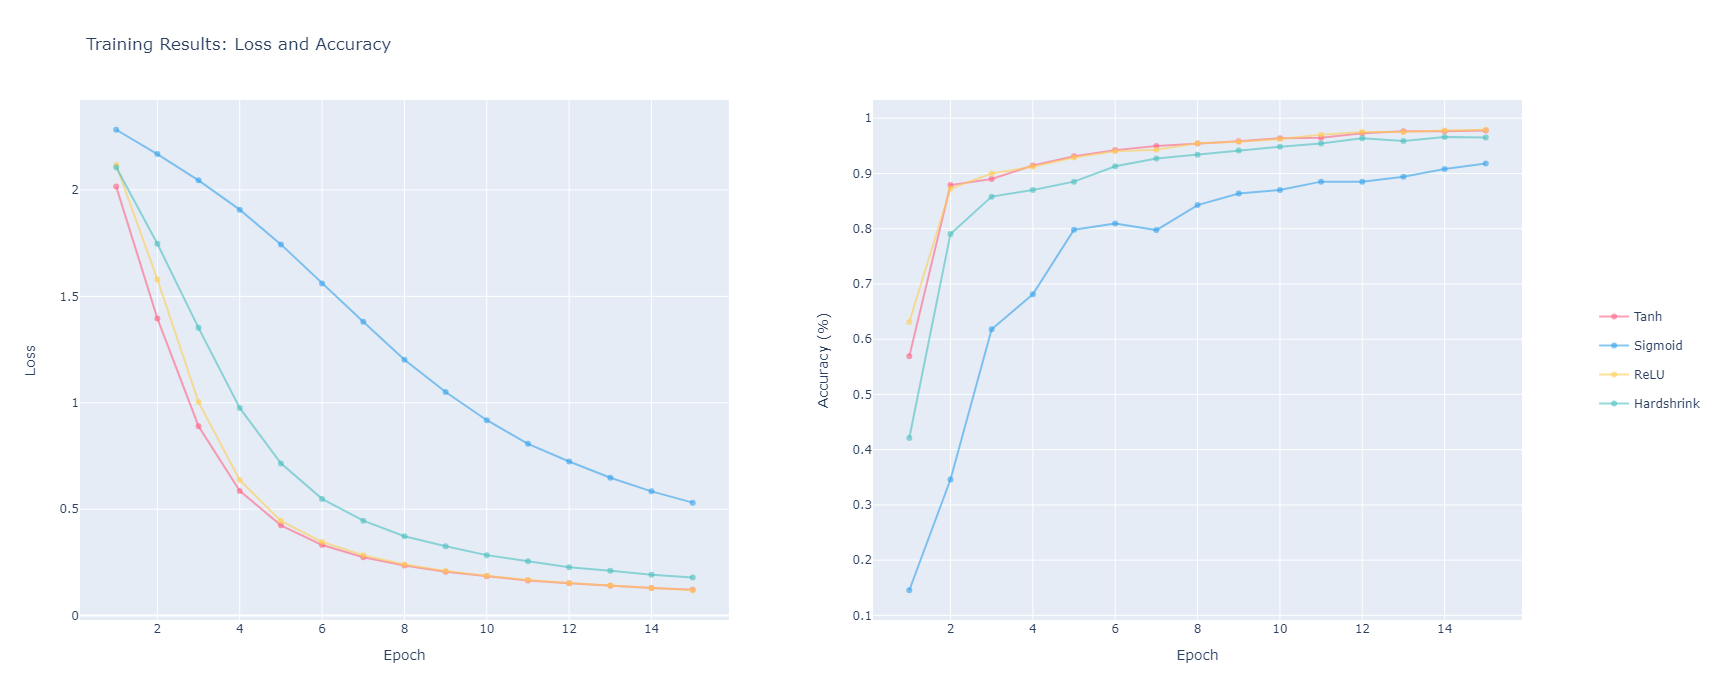
\includegraphics[width=0.9\textwidth]{images/activation_function_loss.png}
    \caption{Effects on model loss and accuracy with different activation functions.}
    \label{fig:activation_function_loss}
\end{figure}

\subsection*{Training Loss}
The performance of various activation functions in terms of training loss is analyzed below:

\begin{itemize}
    \item \textbf{ReLU:} Demonstrates the fastest decline in loss, efficiently handling the gradient flow in the network which supports faster convergence.
    \item \textbf{Tanh:} Shows a moderately quick reduction in loss, indicating good performance but not as efficient as ReLU.
    \item \textbf{Sigmoid:} Exhibits the slowest decline in loss, likely due to issues related to vanishing gradients, especially in deeper network architectures or more complex datasets.
    \item \textbf{Hardshrink:} Performs better than Sigmoid and is nearly on par with Tanh, suggesting potential underexplored benefits in specific contexts.
\end{itemize}

\newpage

\subsection*{Training Accuracy}
The following details the accuracy achieved by different activation functions during training:

\begin{itemize}
    \item \textbf{ReLU:} Achieves the highest accuracy quickly and maintains stable, high performance throughout training, underscoring its effectiveness and robustness across various network settings.
    \item \textbf{Tanh:} Starts slightly slower than ReLU but catches up, maintaining high accuracy nearly matching that of ReLU by the end of the training epochs.
    \item \textbf{Sigmoid:} Mirrors its loss performance with the slowest increase in accuracy, potentially less ideal for tasks requiring quick convergence.
    \item \textbf{Hardshrink:} Competes closely with Tanh and ReLU in terms of accuracy, indicating that when tuned correctly, Hardshrink could be effective in certain applications.
\end{itemize}

\subsection{On the Effects of Network Depth}

\begin{figure}[ht]
    \centering
    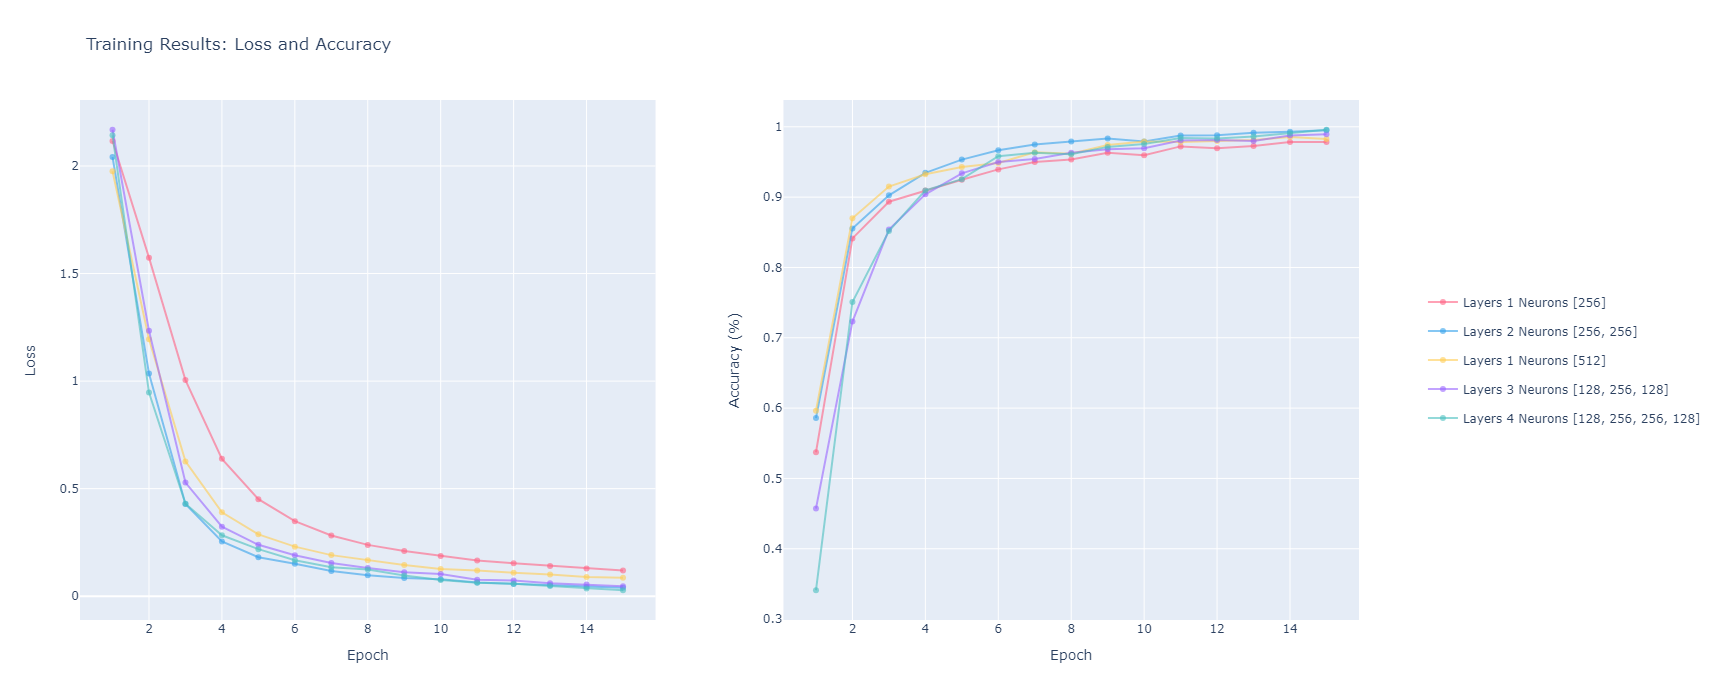
\includegraphics[width=0.9\textwidth]{images/layer_loss.png}
    \caption{Comparison of training loss across different network depths}
    \label{fig:layer_loss}
\end{figure}

\noindent \textbf{Loss Dynamics} \\
Analysis shows that networks with more layers tend to reduce loss more quickly. Specifically, a four-layer configuration ([128, 256, 256, 128])
demonstrates thefastest loss decline, highlighting the efficiency of deeper architectures in handling complex data patterns early in training.
A three-layer setup ([128, 256, 128]) also shows substantial benefits, although slightly less pronounced than the four-layer network.
In contrast, simpler networks like two-layer ([256, 256]) and single-layer ([512]) models exhibit slower initial loss reduction but
ultimately achieve similar loss levels to more complex networks by the end of training.
\vspace*{11pt}

\noindent \textbf{Accuracy Trends} \\
Deeper network architectures consistently outperform shallower ones in terms of accuracy. The four-layer network reaches high accuracy more
quickly and maintains it throughout the training phase, demonstrating superior data processing and generalization capabilities. The three-layer
network also performs well, closely matching the four-layer network’s accuracy, suggesting that increasing layer depth up to a certain point
significantly boosts learning efficiency without the need for very deep structures. Conversely, networks with fewer layers show slower improvement
but eventually reach similar accuracy levels, confirming that less complex networks can still effectively generalize, given sufficient training time.


\end{document}
